\begin{tikzpicture}[scale=1,every node/.style={font=\small}]
\foreach \name/\x/\y/\lab in {a/0/0/{+1},b/2/0/{-1},c/2/2/{+1},d/0/2/{-1}}{
\node[circle,draw=MidnightBlue,fill=white] (\name) at (\x,\y) {$\lab$};}
\draw[MidnightBlue,thick] (a)--(b)--(c)--(d)--(a);
\node[anchor=west,align=left] at (3.2,1) {$Aq=-2q$\\$(A/2)q=-q$\\$\tfrac12(I+A/2)q=0$};
\end{tikzpicture}
